% ------------------------------------------------------------------------ %
% !TEX encoding = UTF-8
% !TEX TS-program = pdflatex
% !TEX root = ../Project.tex
% !TEX spellcheck = en-EN
% ------------------------------------------------------------------------ %
%
% ------------------------------------------------------------------------ %
% 	CHAPTER TITLE
% ------------------------------------------------------------------------ %
%
\chapter{User Interface Design}
%
\label{cap:userinterfacedesign}
%
%
This section is a recapitulation of the section 3.B.1 (User Interfaces) of the Requirements Analysis and Specification Document and a deepening of design aspects of the user interface.
The application will be developed as a mobile application for the main mobile operating systems (iOS and Android).
As the system will appear the same for all the users, it will provide all the functionalities described in the RASD, in a unique user interface.
%
%
% ------------------------------------------------------------------------ %
%
%
\section{Mockups}
Following some mockups will provide an idea of the user interface while the user interacts with it, making use of the functionalities of the application. It includes most of the main screen that the user will face.

\begin{center}

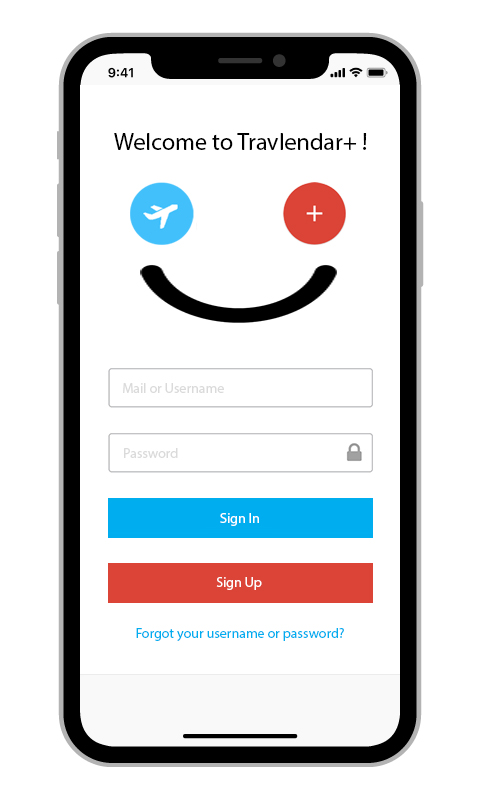
\includegraphics[scale=2.4]{MainMatter/images/ui/login}
\captionof{figure}{Mockup of the login screen}

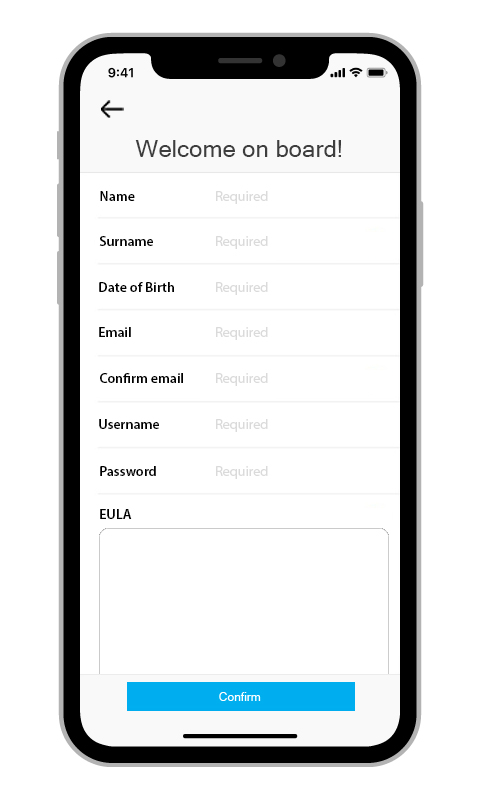
\includegraphics[scale=2.4]{MainMatter/images/ui/signup}
\captionof{figure}{Mockup of the registration screen}

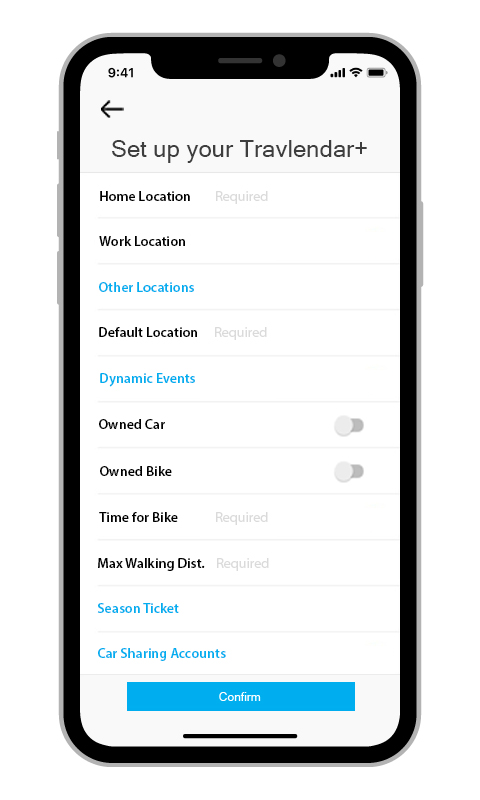
\includegraphics[scale=2.4]{MainMatter/images/ui/firstsetup}
\captionof{figure}{Mockup of the screen where the user can set his preferences}

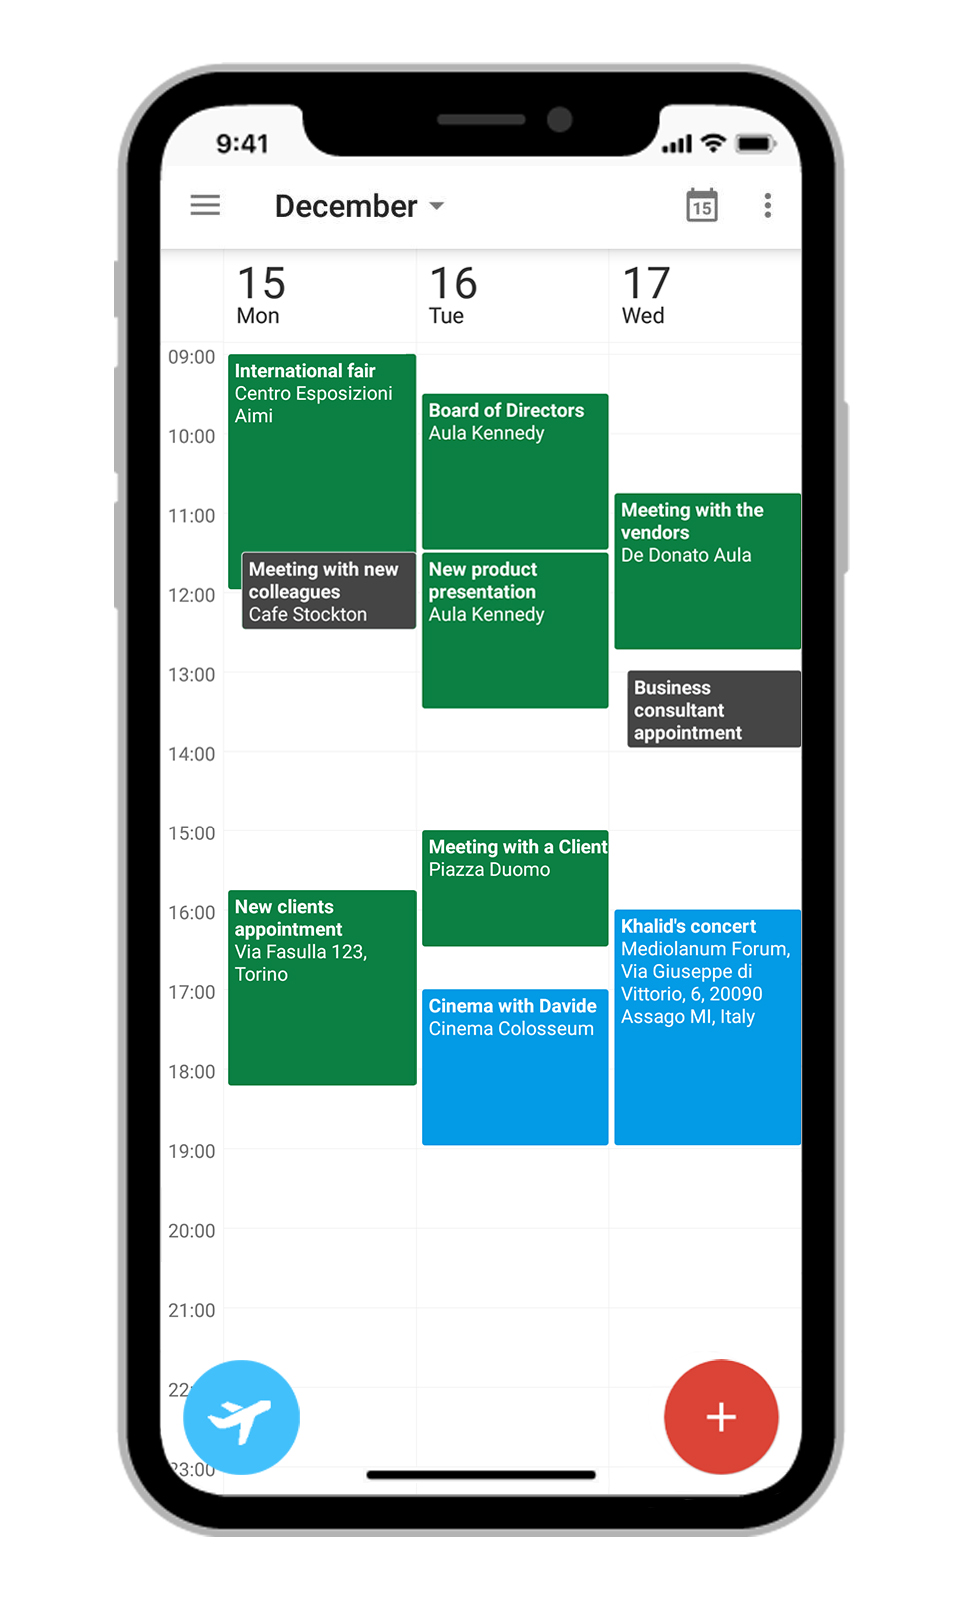
\includegraphics[scale=1.2]{MainMatter/images/ui/calendar}
\captionof{figure}{Mockup of the calendar screen with primary and secondary events}

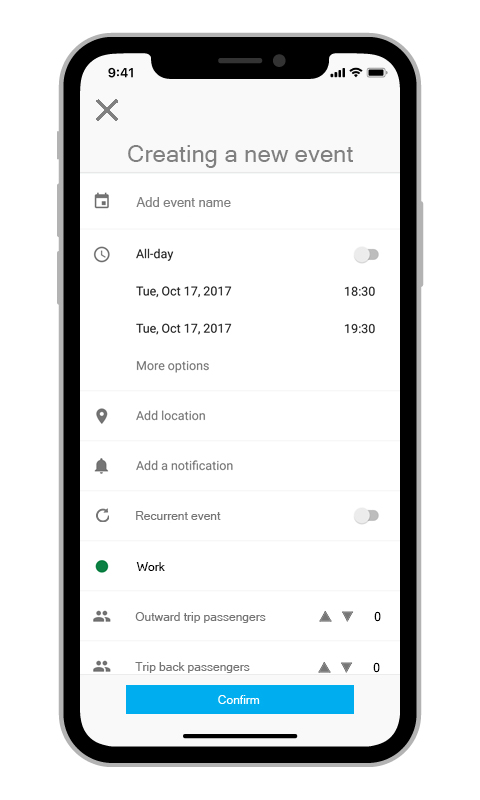
\includegraphics[scale=2.4]{MainMatter/images/ui/newevent}
\captionof{figure}{Mockup of the screen that allows to add an event}

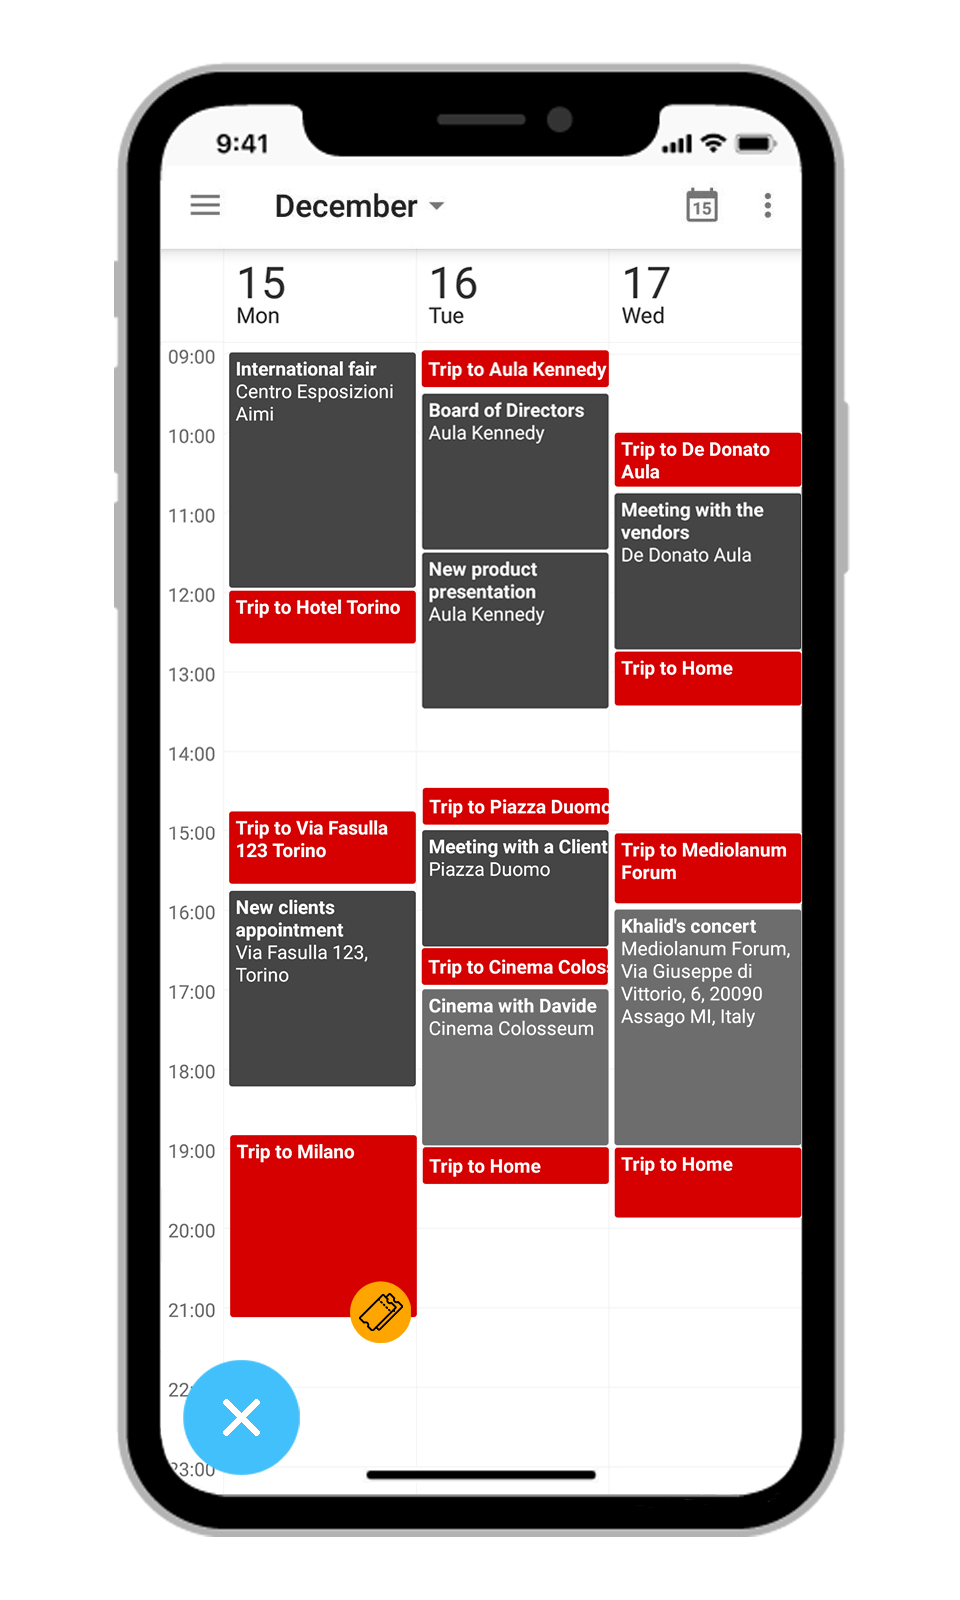
\includegraphics[scale=1.2]{MainMatter/images/ui/tripscreen}
\captionof{figure}{Mockup of the screen with the trips shown}

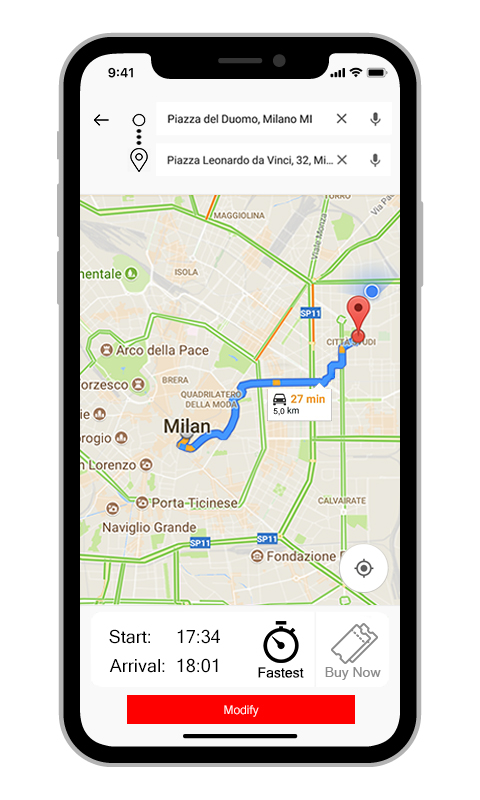
\includegraphics[scale=2.4]{MainMatter/images/ui/journeydetails}
\captionof{figure}{Mockup of the trip details screen}

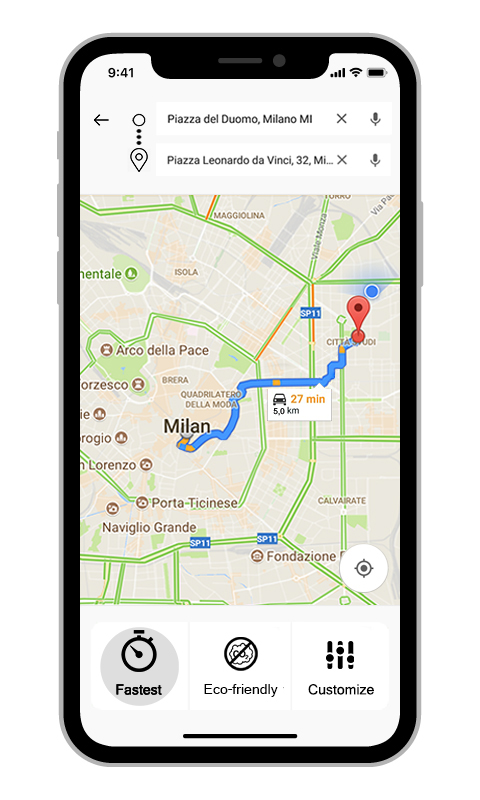
\includegraphics[scale=2.4]{MainMatter/images/ui/journeychoose}
\captionof{figure}{Mockup of the screen that allows the user to modify a trip}

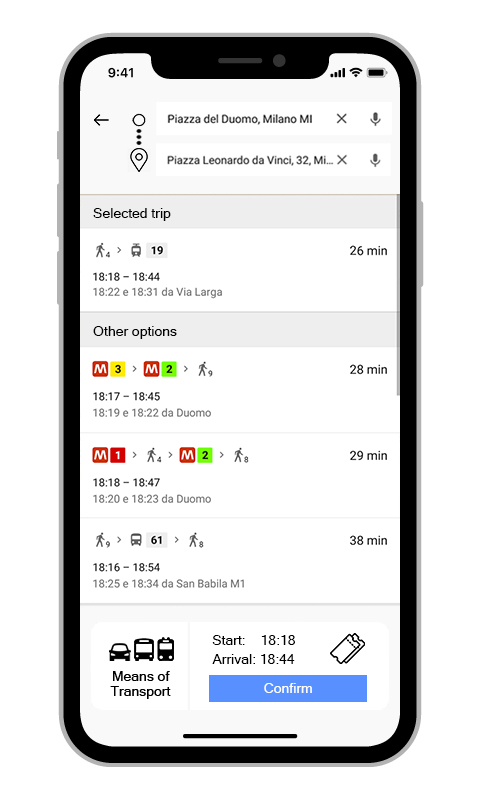
\includegraphics[scale=2.4]{MainMatter/images/ui/customized}
\captionof{figure}{Mockup of the screen with the customization of a trip}

\end{center}
%
%
% ------------------------------------------------------------------------ %
%
%
\section{UX Diagrams}
UX diagrams provide information about the user interface of the system and how the user interacts with it.
For the diagram comprehension purposes, additional screens used to add specific information (other locations, dynamic events, season tickets, etc…) in the preferences setup are not considered.

\begin{center}
\makebox[\textwidth][c]{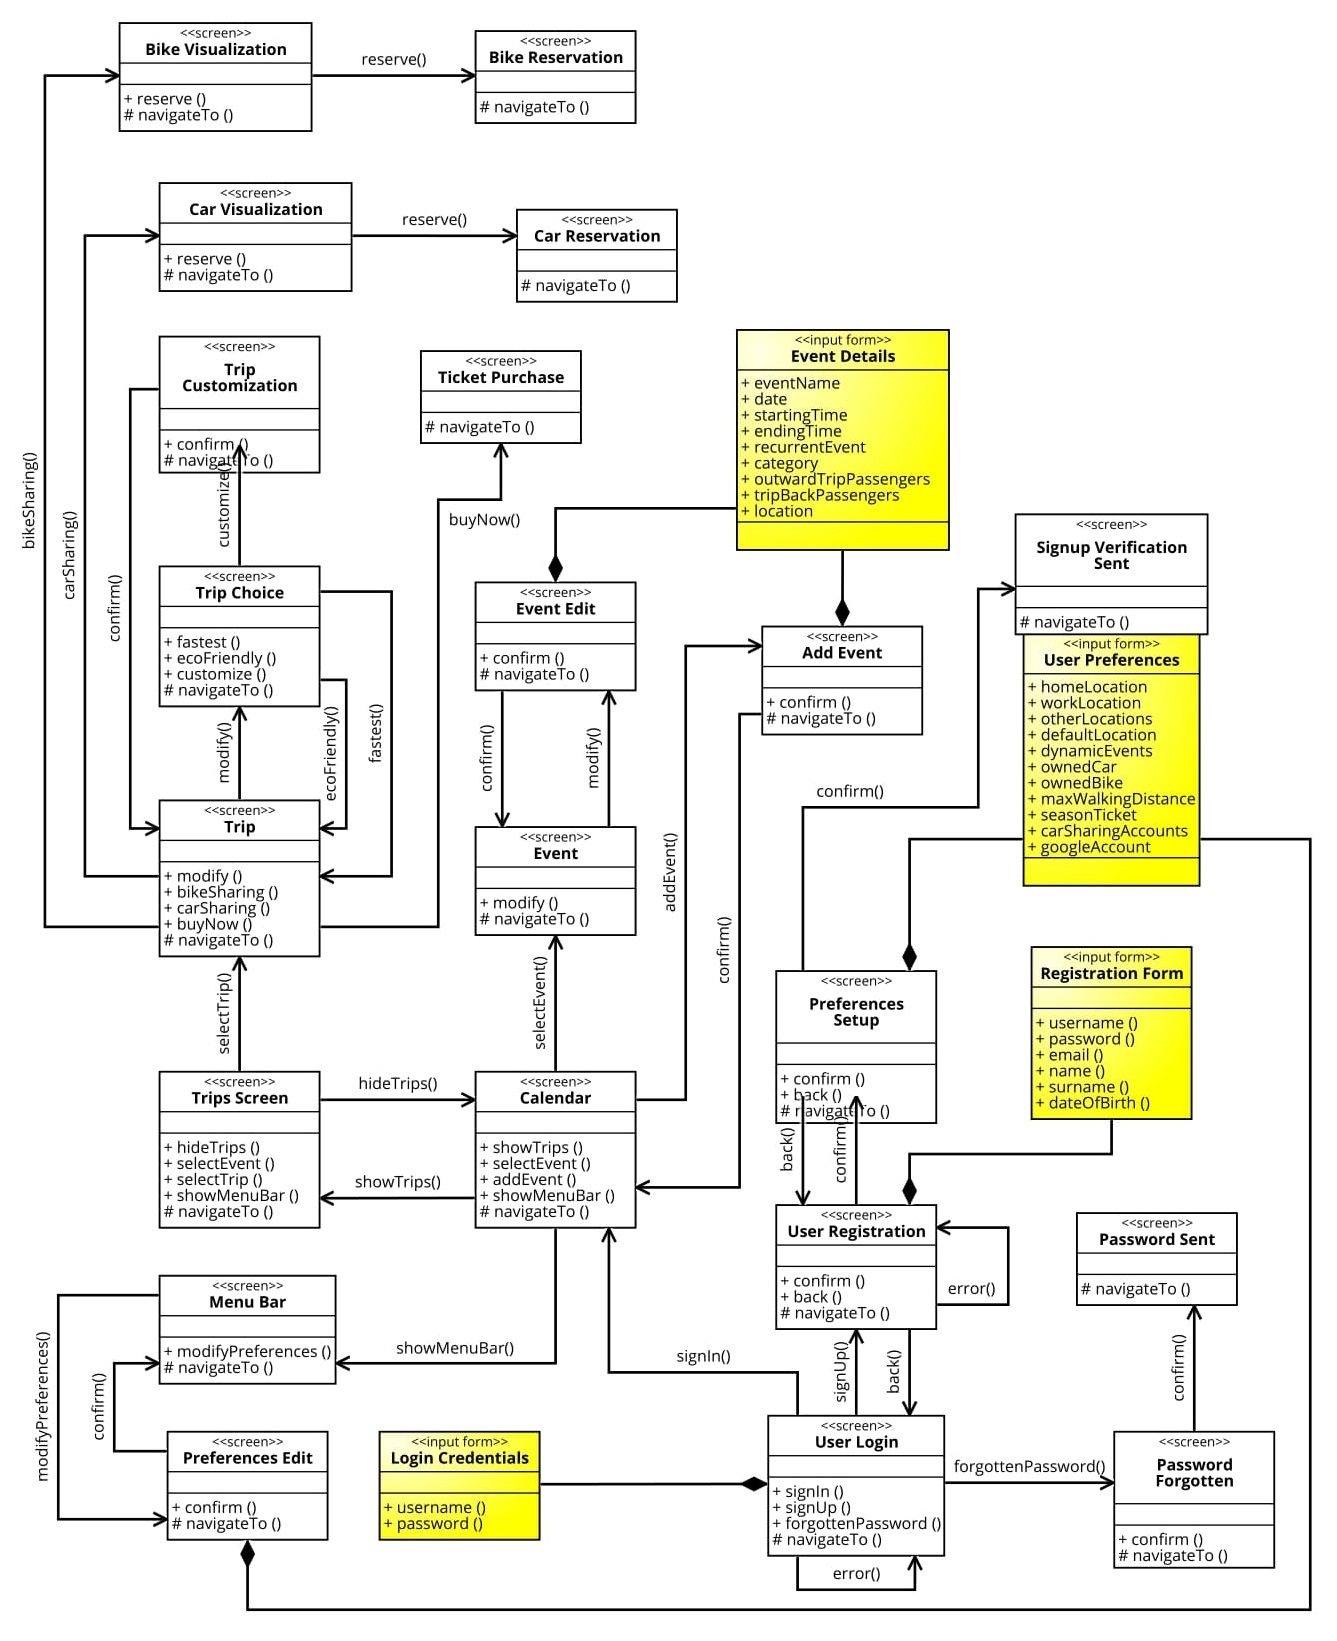
\includegraphics[width=1.15\textwidth]{MainMatter/images/ui/ux}}
\captionof{figure}{UX diagram of the application}
\end{center}
%
%
% ------------------------------------------------------------------------ %
%
%
\section{BCE Diagrams}
For the implementation of the system, a Model-View-Controller design pattern is adopted and BCE diagrams are useful to show how user interactions are managed internally by the system. Boundaries are objects that interface with the users of the application; Entities object model the access to data; Controls object manage the communication between boundaries and entities.

\begin{center}
\makebox[\textwidth][c]{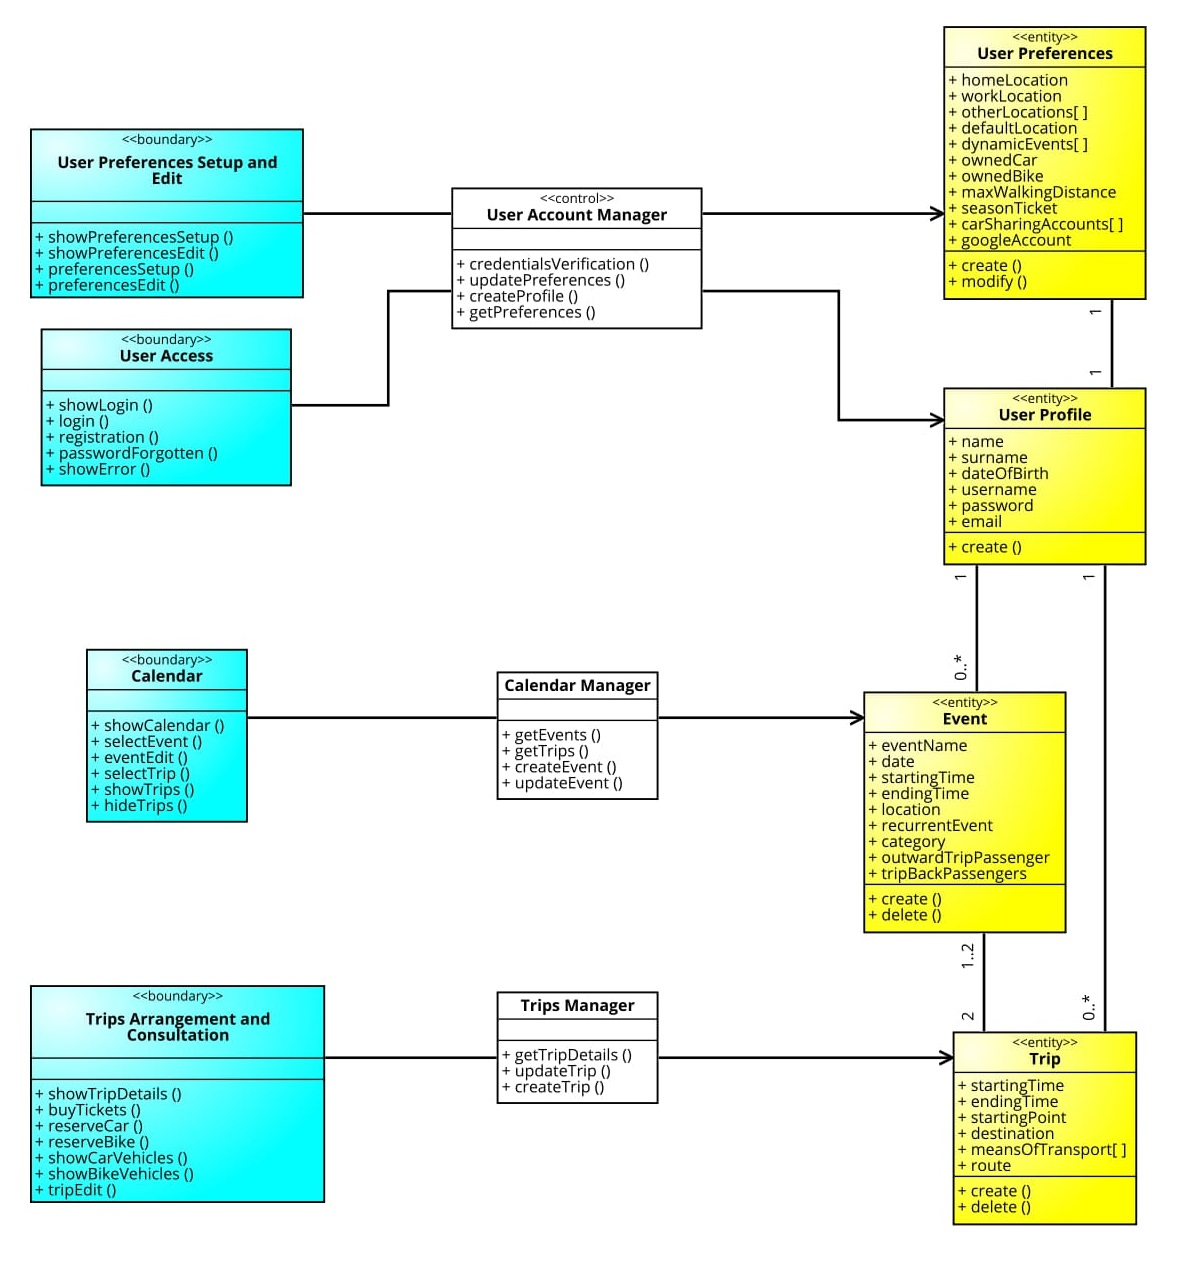
\includegraphics[width=1.1\textwidth]{MainMatter/images/ui/bce}}
\captionof{figure}{BCE diagram of the application}
\end{center}
%
%
% -----------------------------END------------------------------------- %
